\chapter{ADC Control Measurements} \label{App:ADCControlMeasurement}
In order to test the ADC control hardware, a PCB has been made that connects the FPGA and LTC2311 ADC. This can be seen on figure \refq{fig:A_ADC_CONTROL_MEAS_SETUP}.

\begin{figure}[H]
    \centering
    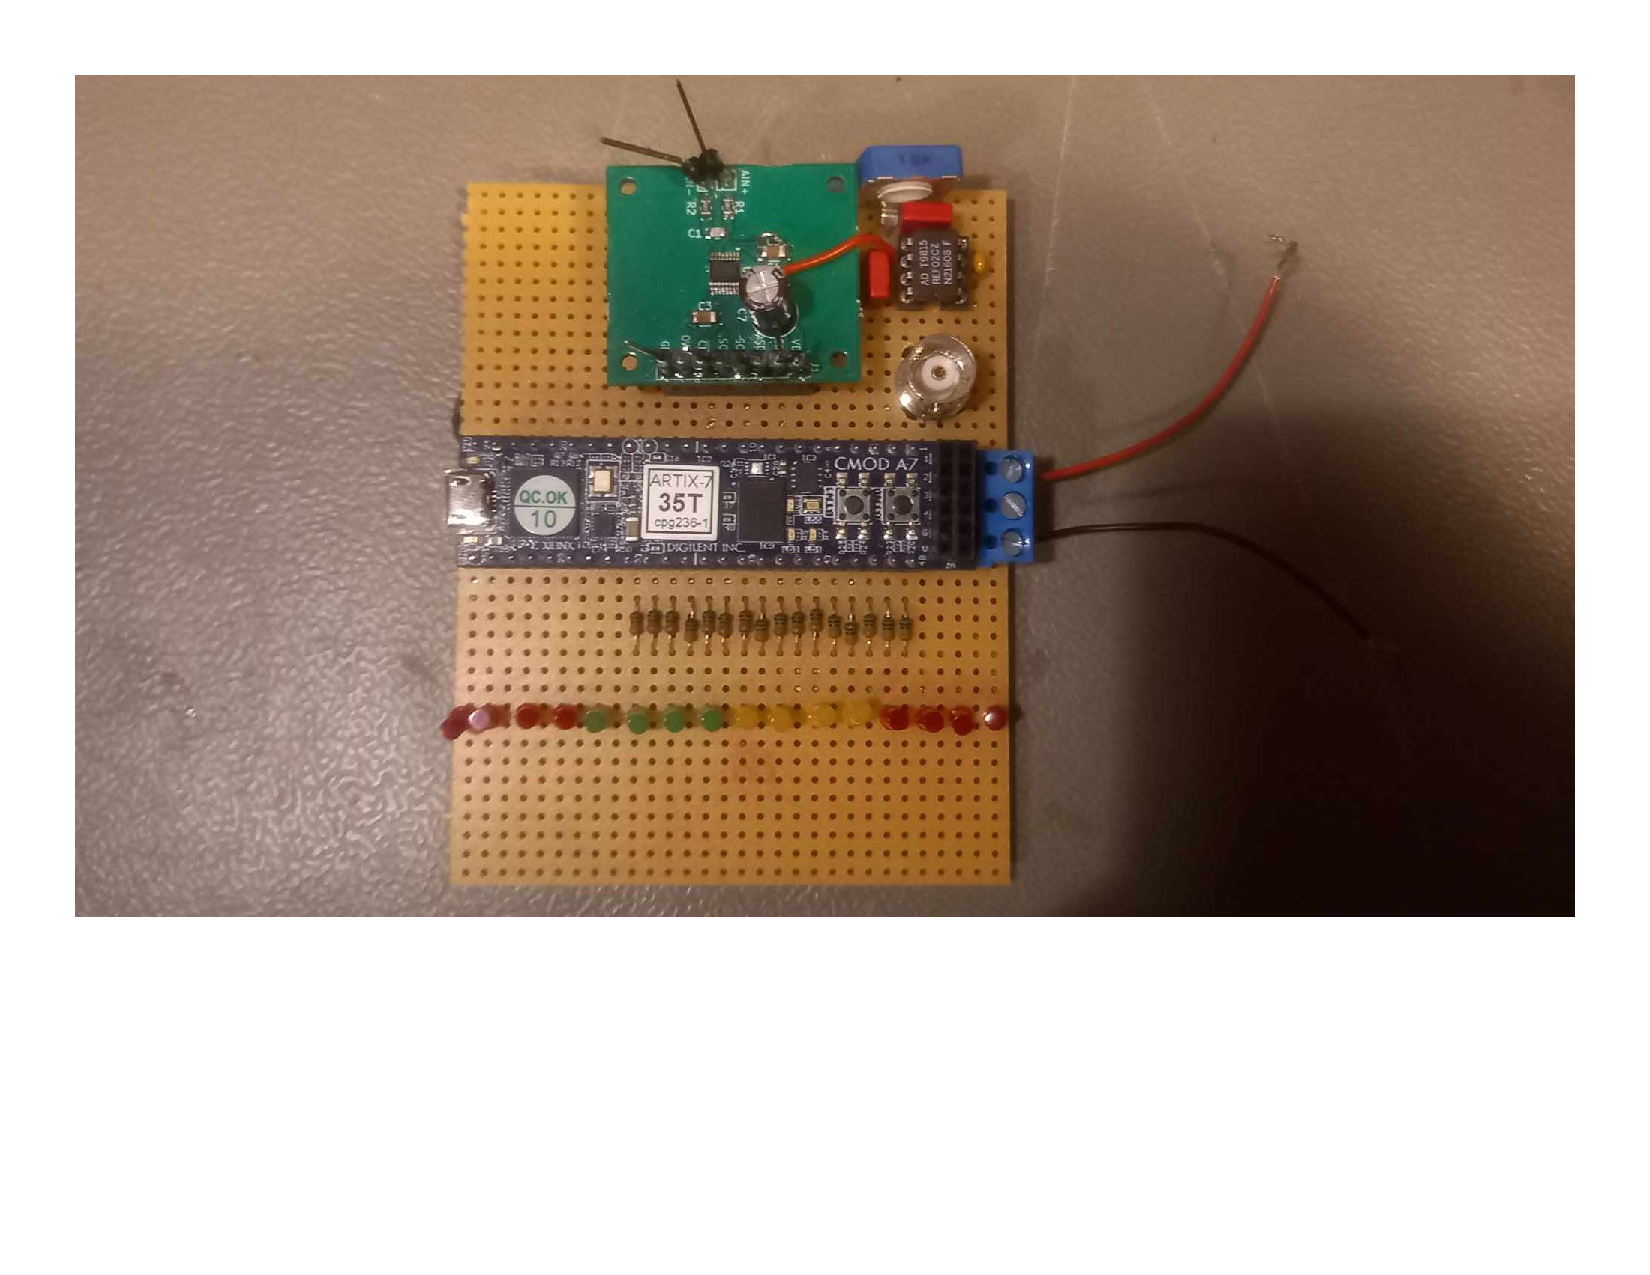
\includegraphics[clip, trim=0 100 0 0, width=0.9\textwidth]{Appendix/Figures/A_ADC_CONTROL_MEAS_ADC Control Tesr Setup.pdf}
    \caption{A PCB for testing the ADC Control module. The Artix 7 FPGA, in the middle, is connected to the LTC2311 ADC, in the top. The ADC input is connected to a potentiometer in order to set the voltage it will read. The actual ADC reading can be read on the 16 LEDs in the bottom of the board.}
    \label{fig:A_ADC_CONTROL_MEAS_SETUP}
\end{figure}

The board in the middle is the CMOD A7 Artix 7 development board being used in the project. The connections to the FPGA is not interesting as all FPGA pins can be used as GPIO, so, any pins can be chosen here. While the green board in the top is a break out board for the LTC2311 ADC that was designed for this project. The schematic for this breakout board can be seen on figure \refq{fig:A_ADC_CONTROL_LTC2311SCH}

\begin{figure}[H]
    \centering
    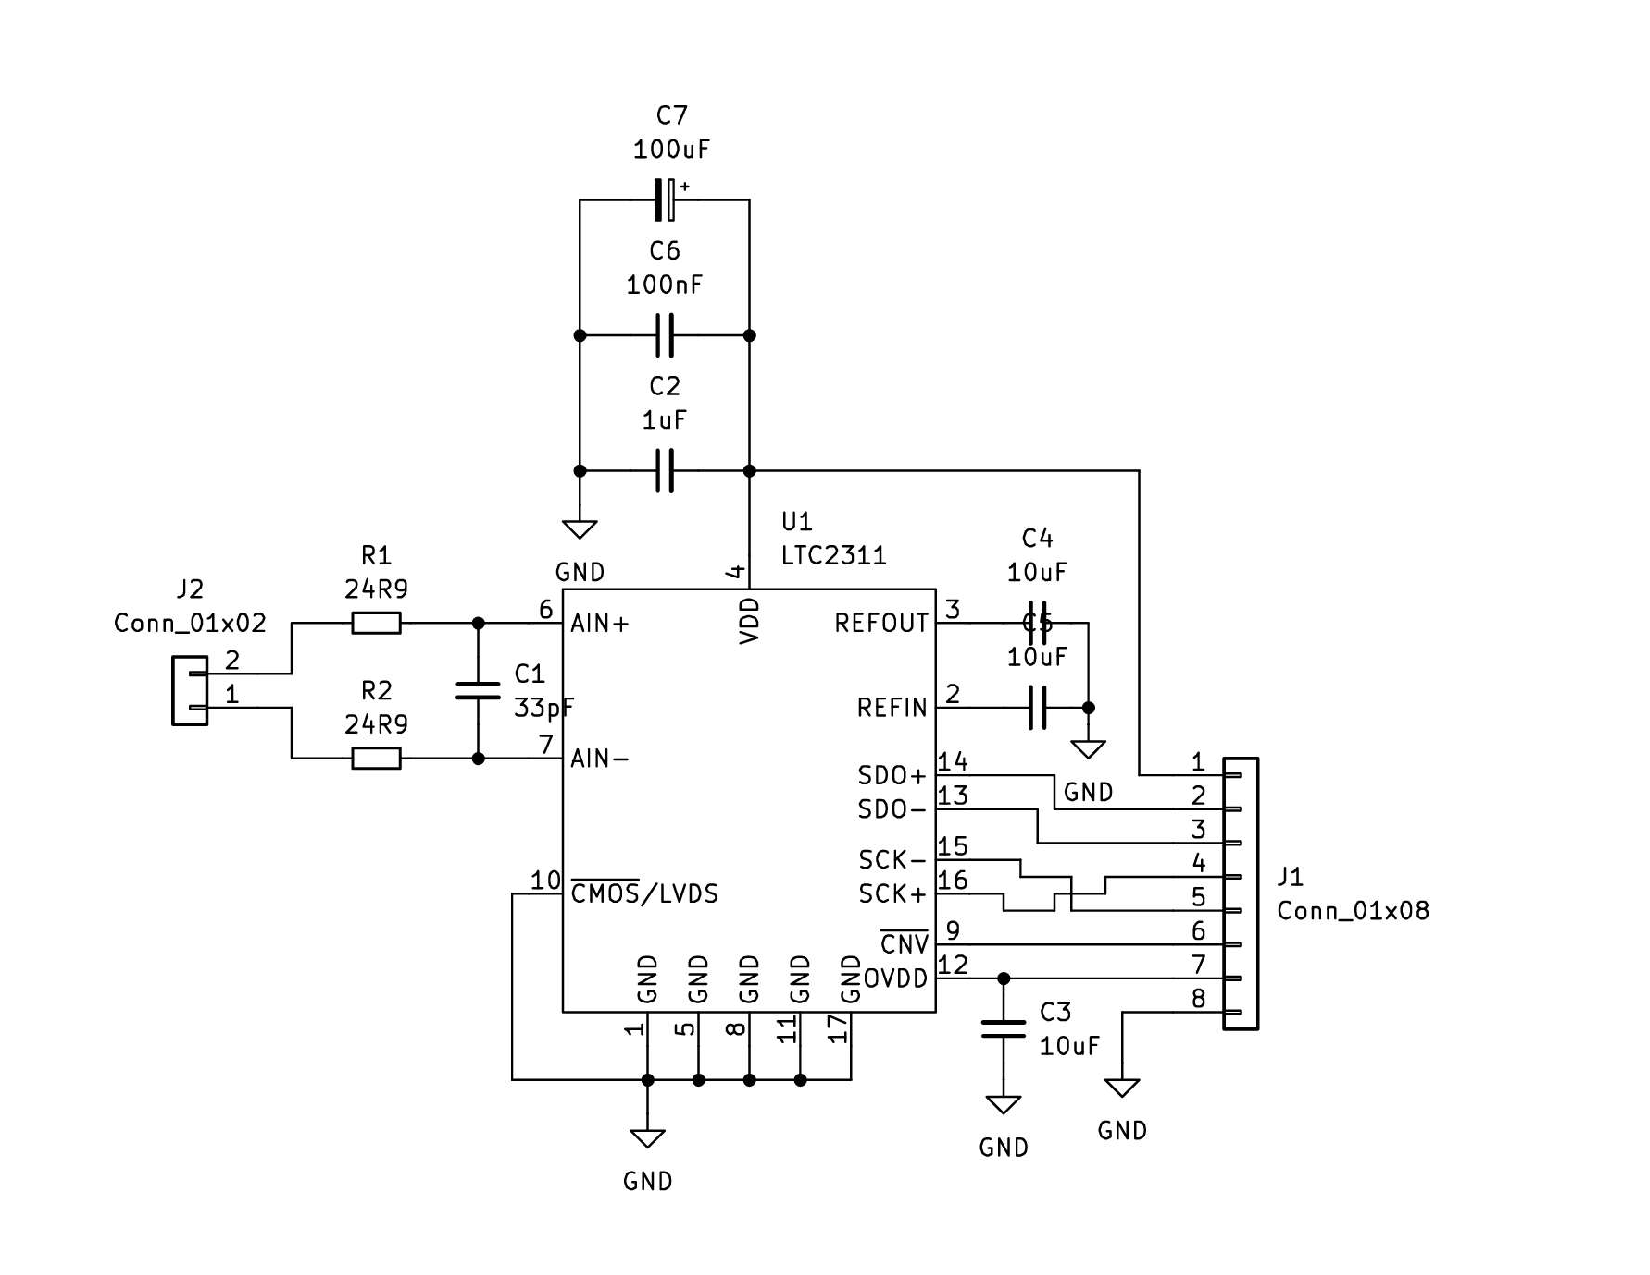
\includegraphics[clip, trim=0 0 0 0, width=1\textwidth]{Appendix/Figures/A_ADC_CONTROL_LTC2311SCH.pdf}
    \caption{The schematic for the LTC2311 ADC Breakout board that was designed for this project.}
    \label{fig:A_ADC_CONTROL_LTC2311SCH}
\end{figure}

Note how the LTC2311 is being used in "CMOS" mode as can be sen on figure \refq{fig:A_ADC_CONTROL_LTC2311SCH}. This means the communication for the LTC2311 is single ended. Setting the CMOS/LVDS mode changes the LTC2311 to LVDS mode which means the SCK and SDO signals will be in differential mode.

The BNC connector on figure \refq{fig:A_ADC_CONTROL_MEAS_SETUP} is an input that can be used as a manual, external, trigger input for the ADC control block. The LEDs on the bottom can be used to see an actual reading from the ADC. The accuracy of the readings are not interesting here as the module only controls the timing and communication between the LTC2311 and the FPGA.

The signal going to the CNV pin has been measured and can be seen on figure \refq{fig:A_ADC_CONTROL_CNV}.

\begin{figure}[H]
    \centering
    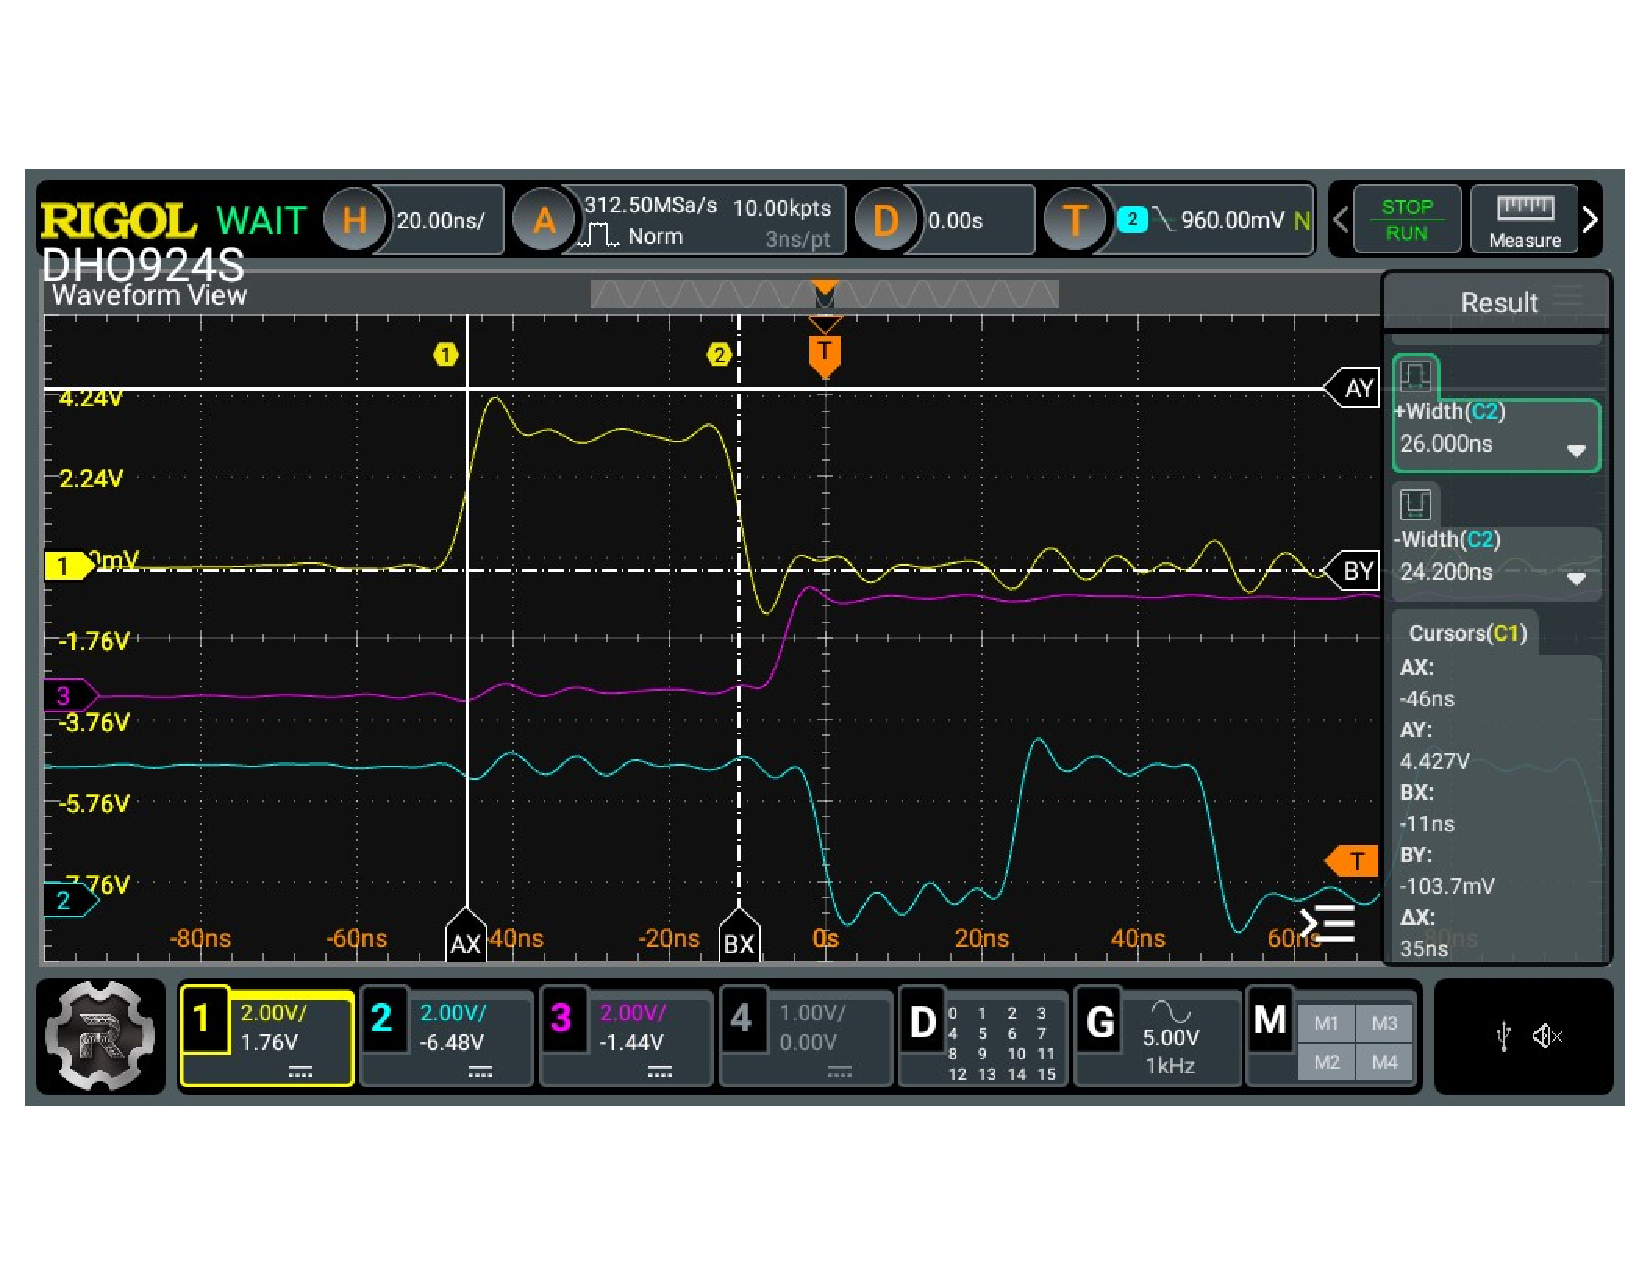
\includegraphics[clip, trim=0 75 0 0, width=1\textwidth]{Appendix/Figures/A_ADCControl_CNV_MEASURE.pdf}
    \caption{A measurement of the pulse width of the CNV pin signal. The pulse width is \SIQ{35}{\nano\second} as expected. The yellow trace is CNV. The purple trace is ADC data and the blue trace is SPI CLK.}
    \label{fig:A_ADC_CONTROL_CNV}
\end{figure}

The CNV to CLK signal dead time has been measured and can be seen on figure \refq{fig:A_ADC_CONTROL_DCN}.

\begin{figure}[H]
    \centering
    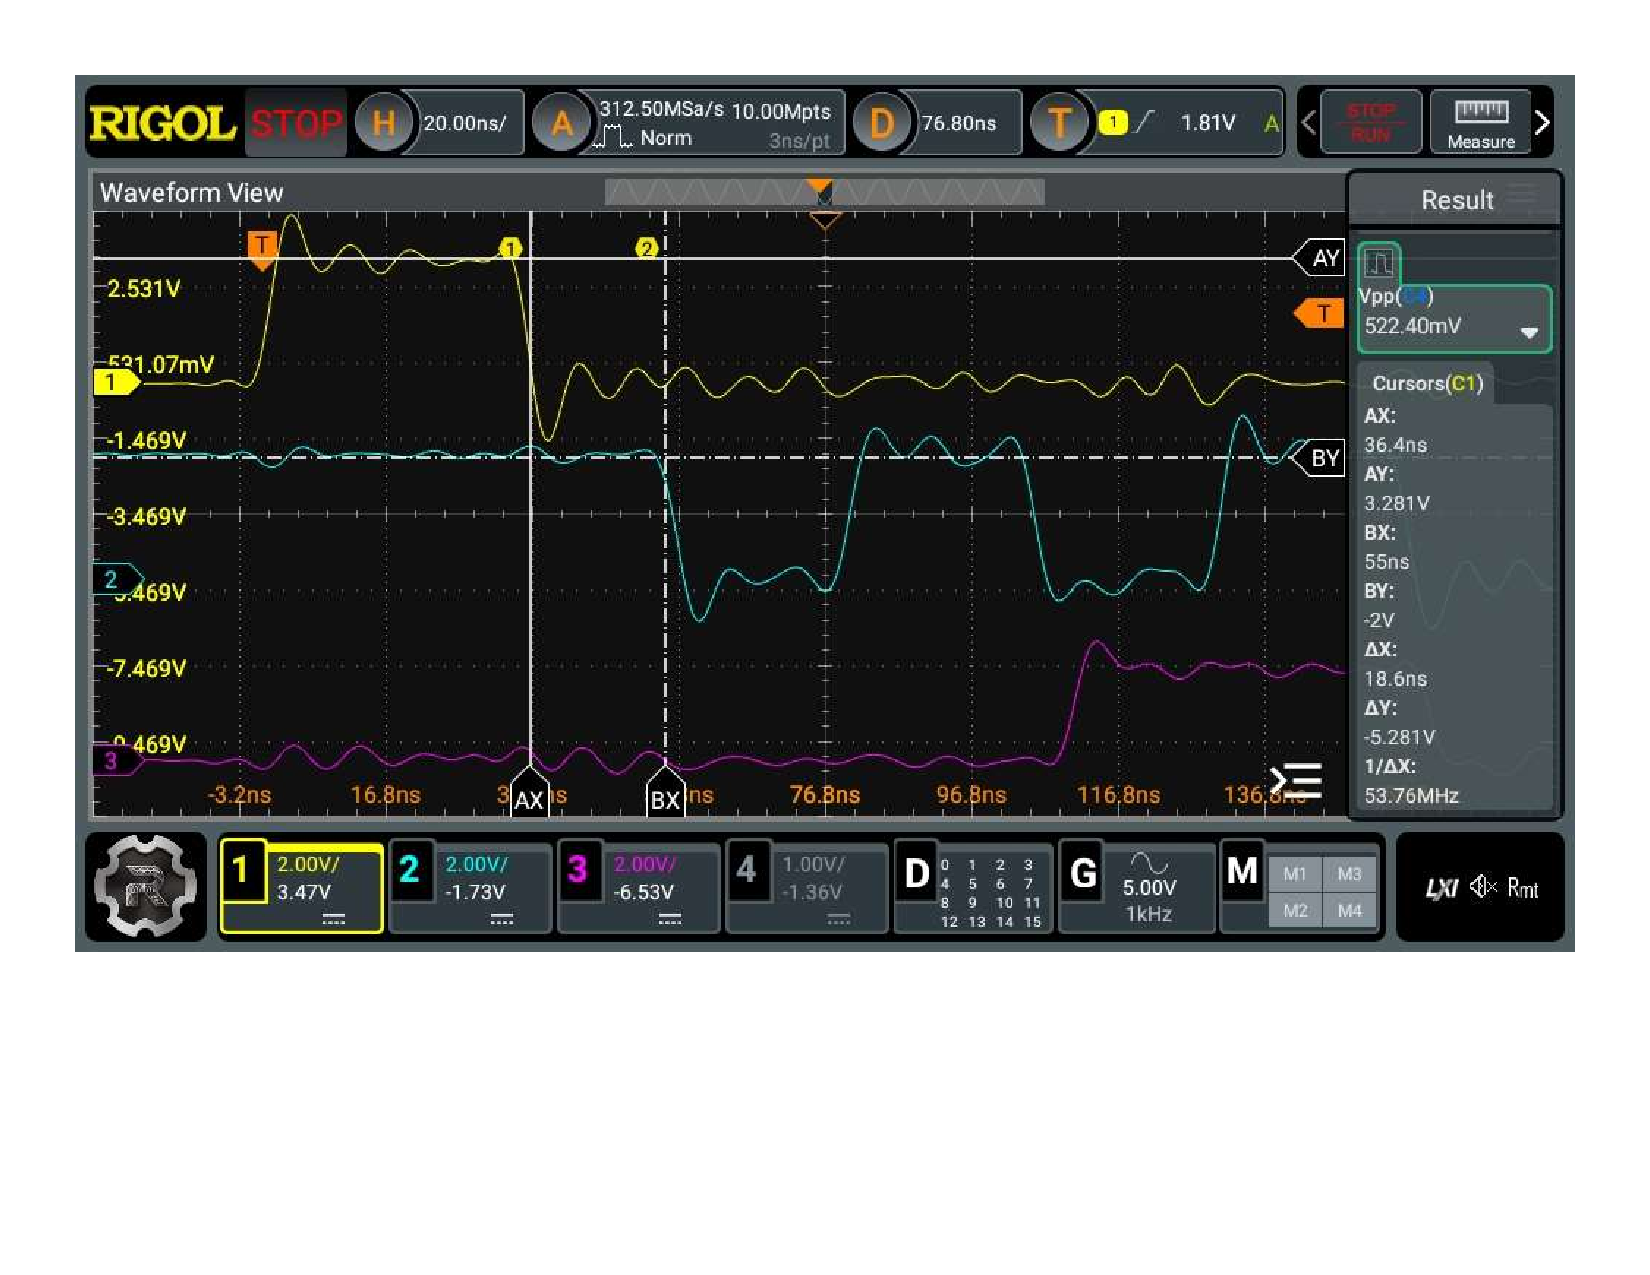
\includegraphics[clip, trim=0 150 0 0, width=1\textwidth]{Appendix/Figures/A_ADC_CONTROL_DCN_MEAS.pdf}
    \caption{A measurement of the dead time between the falling edge of the CNV pin signal and the start of the SPI CLK. The dead time is about \SIQ{18.6}{\nano\second} which is OK for this project.  The yellow trace is CNV. The purple trace is ADC data and the blue trace is SPI CLK.}
    \label{fig:A_ADC_CONTROL_DCN}
\end{figure}

The pulse widths of the SPI CLK signals have been measured and this can be seen on figure \refq{fig:A_ADC_CONTROL_SPICLKWIDTH}.
\begin{figure}[H]
    \centering
    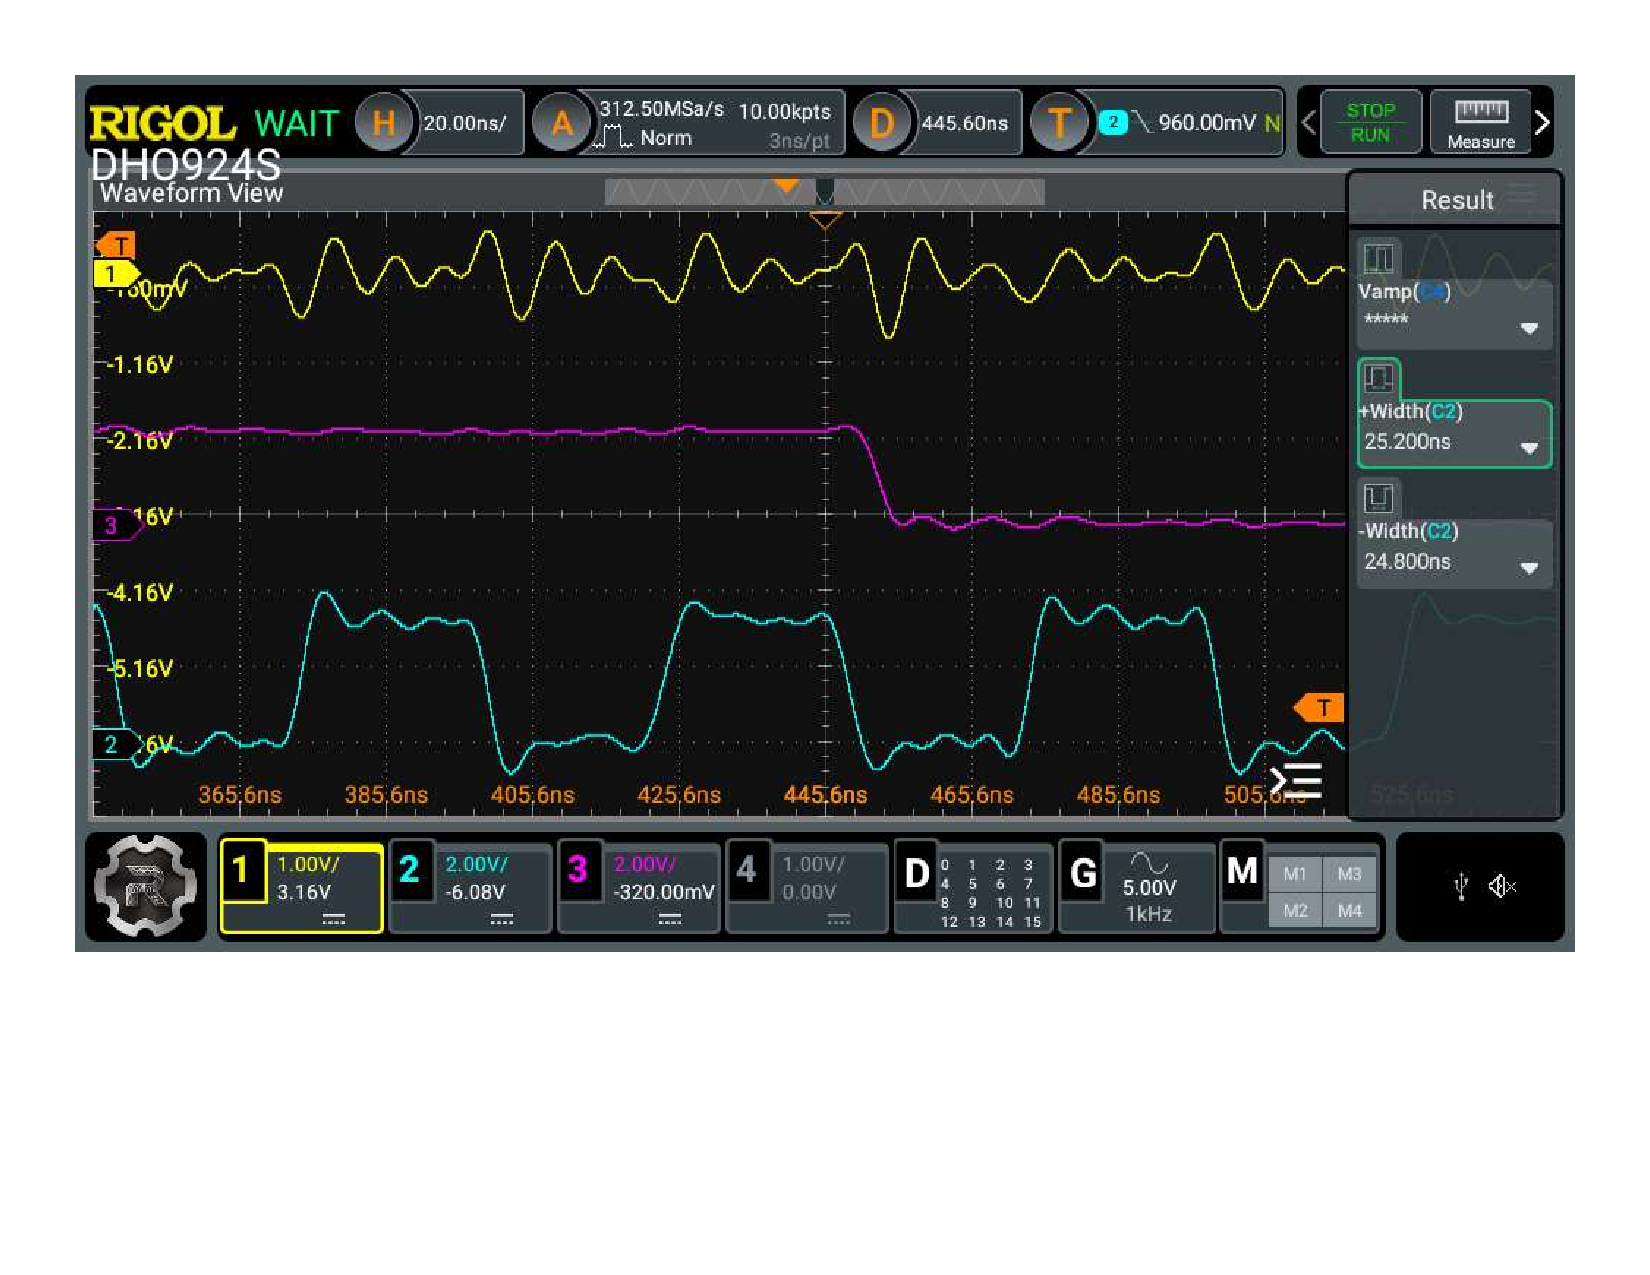
\includegraphics[clip, trim=0 150 0 0, width=1\textwidth]{Appendix/Figures/A_ADC_CONTROL_PULSEWIDTH.pdf}
    \caption{A measurement of pulse widths of the SPI CLK pulses can be seen. Both the high and low time is about \SIQ{25}{\nano\second} as was expected for this.  The yellow trace is CNV. The purple trace is ADC data and the blue trace is SPI CLK.}
    \label{fig:A_ADC_CONTROL_SPICLKWIDTH}
\end{figure}

The SPI CLK frequency can also be seen on figure \refq{fig:A_ADC_CONTROL_SPICLKWIDTH} and is \SIQ{20}{\mega\hertz}. It was checked whether the ADC control can do 1 MS/s and this test can be seen on figure \refq{fig:A_ADC_CONTROL_1MSS}.

\begin{figure}[H]
    \centering
    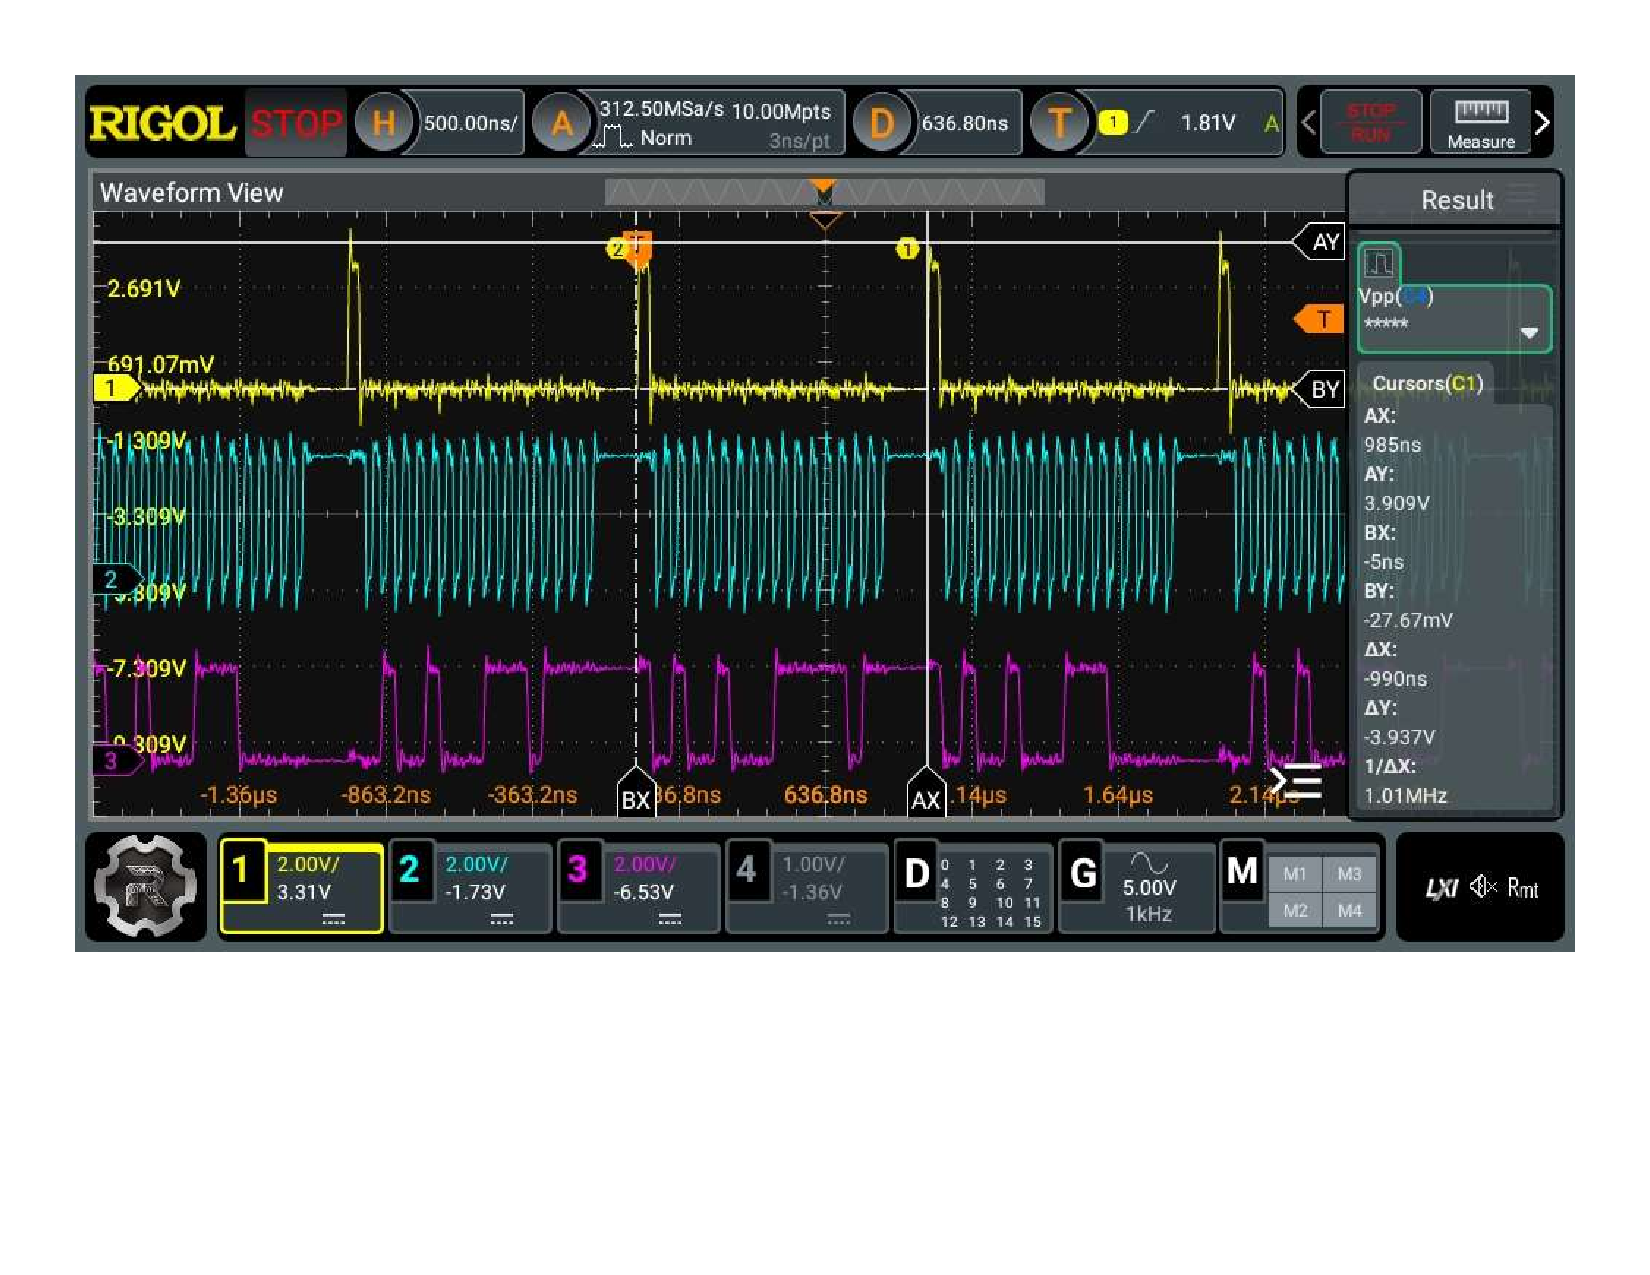
\includegraphics[clip, trim=0 150 0 0, width=1\textwidth]{Appendix/Figures/7_2_8_ADC_CONTROL_1MEGSAMPLE_MEAS.pdf}
    \caption{A test of the ADC control block running at 1 MS/s. There are no glitches in the communication so the hardware works at 1 MS/s. The yellow trace is CNV. The purple trace is ADC data and the blue trace is SPI CLK.}
    \label{fig:A_ADC_CONTROL_1MSS}
\end{figure}